\chapter{Revisión de la Tecnología Blockchain y sus aplicaciones}\label{chapter:state-of-the-art}

En este primer capítulo, se pretende explicar el estado de las tecnologías blockchain, en las que se basa el tema central de este proyecto.
Se hace un análisis de sus orígenes para poder comprender su evolución.
Además, se detalla sobre el framework que será usado para la solución.
Finalmente se hace un estudio sobre trabajos con un objetivo similar al de este proyecto.

\section{Conceptos fundamentales de la Tecnología Blockchain Aplicada}

Esta sección presenta una visión general de la tecnología blockchain e introduce las características principales como sistema de almacenamiento de datos descentralizado, confiable e inmutable.

\subsection{Los orígenes}

El dinero es un medio de cambio a través del cual se adquieren bienes y servicios o se utiliza para el pago de obligaciones. Todos los días se asocia un precio a los objetos de acuerdo con su valor intrínseco y a otros factores, como su disponibilidad (oferta) y las necesidades de las personas (demanda). Su representación ha cambiado a lo largo del tiempo: hojas de árboles raros, minerales preciosos o certificados bancarios. Todas sus representaciones cumplen que son raras de obtener y difíciles de imitar. Cuando se encuentra una forma de generar esta representación sin tener respaldo en bienes y servicios entonces este pierde su capacidad de compra.

Desde la aparición de los ordenadores personales y posteriormente de Internet se ha intentado crear una forma digital de representación del dinero que mantenga su valor y complemente(incluso desplace) las formas de intercambio actual. No es hasta que se desarrollaron una serie de tecnologías independientes como la criptografía de clave pública, las blockchain, las redes `peer-to-peer' y el  `timestamping' que fue posible encontrar esta representación digital.

En la década de los 90 del siglo pasado aparecen diferentes trabajos sobre soluciones descentralizadas para realizar pagos electrónicos que no dependan de la intervención de ninguna entidad central supervisora ni reguladora.

En 1991 aparece el primer trabajo de una cadena de bloques segura utilizando criptografía[\cite{200}] que fue evolucionando hasta que en 1998, Wei Dai[\cite{201}] describe una solución descentralizada para pagos electrónicos basada en criptografía de clave pública. Este primer trabajo es evolucionado por otros autores hasta que en 2008 se publica, con el pseudónimo de Satoshi Nakamoto, el artículo "Bitcoin: A Peer-to-Peer Electronic Cash System" [\cite{nakamoto2008bitcoin}] que define el mecanismo para implementar una moneda digital: Bitcoin. Este se basa en el uso de las cadenas de bloques (blockchain) para registrar las transacciones en una red peer-to-peer.

\subsection{Aplicaciones de blockchain}
Durante la última década, la aplicación de blockchain se ha extendido a otras áreas, que trascienden el dinero y las criptomonedas, como las finanzas, la salud, la educación, el encadenamiento productivo, la gobernanza. Algunas de las aplicaciones generales transversales que pueden ser implementadas de manera universal son: la identidad digital y la trazabilidad verificable.

Con una identidad digital cada usuario puede elegir qué información de sí mismo mantiene de manera pública o privada ante terceros. Los smart contracts o contratos inteligentes son acuerdos digitales que se realizan entre dos o más partes. Estos contratos se ejecutan de manera automática cuando se cumple determinada condición aceptada previamente por las partes involucradas. Como toda la información registrada en la blockchain queda distribuida e inalterable, esta tecnología permite que se pueda realizar tracking o seguimiento a ciertos registros específicos. De este modo, los usuarios pueden ver los detalles de las transacciones o actualizaciones relacionadas con un elemento en particular.

\subsection{Características básicas}
De manera sintetizada una blockchain se define como un sistema de almacenamiento descentralizado, distribuido e inmutable: [\cite{zheng2017overview}][\cite{makridakis2019blockchain}].
\begin{itemize}
	\item Descentralización: No se necesita confiar en una sola entidad, sino que se distribuyen las responsabilidades entre múltiples o todos los nodos.
	\item Inmutabilidad: Una vez que un número suficiente de participantes de la blockchain aceptan los datos y los agregan, la información se almacena de forma permanente e inmutable.
	\item Consenso: Es el proceso de acordar la validez de las transacciones entre un número suficiente de participantes de la red.
	\item Escalabilidad: En caso de incrementarse la cantidad de participantes drásticamente puede mantener la velocidad de sus transacciones modificando los mecanismos de consenso y/o el tamaño de los bloques de datos.
	\item Validez y seguridad de los datos: La combinación de consenso e inmutabilidad da como resultado la capacidad de validar y proteger los datos.
	\item Privacidad controlada: La privacidad depende del tipo de blockchain. Los datos pueden ser visibles para todos los participantes o limitados a un grupo específico.
\end{itemize}

\subsection{Clasificaciones de Blockchain}

\begin{figure}[h!]
	\centering
	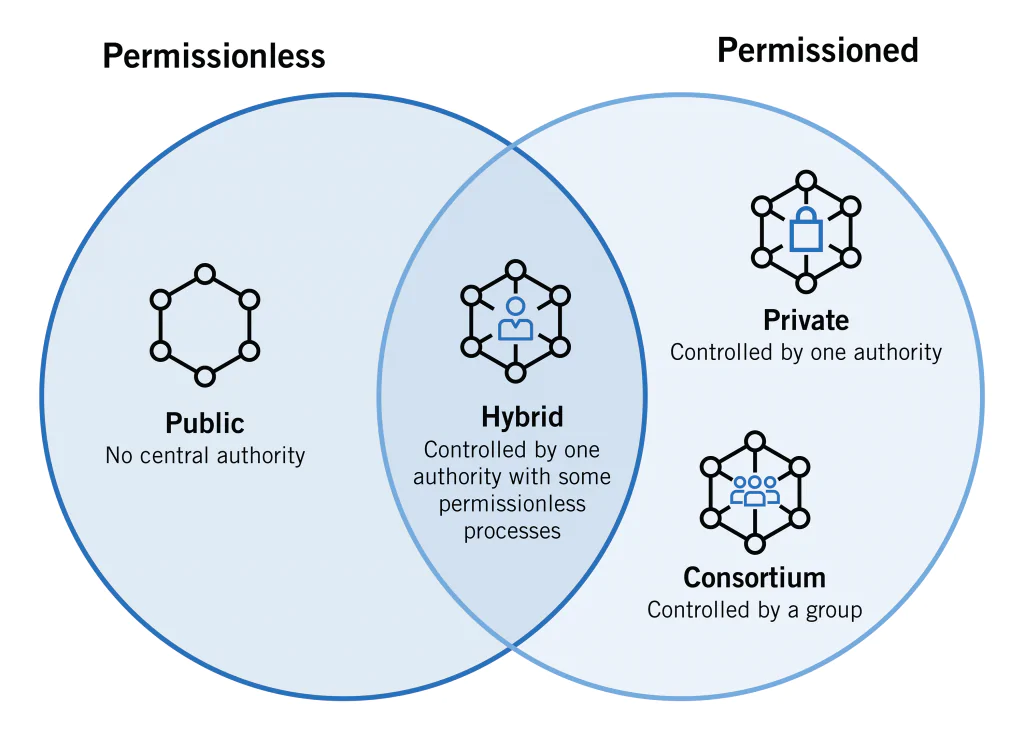
\includegraphics[width=\linewidth]{Graphics/bc_types.png}
	\caption{Tipos de Blockchain}
	\label{fig:1}
\end{figure}

Para implementar una aplicación basada en blockchain, se deben considerar los tipos existentes de blockchain en cuanto a su privacidad (Figura \ref{fig:1}) [\cite{alhadhrami2017introducing}]:
\begin{itemize}
	\item Público: La red está completamente descentralizada y no requiere permisos para participar. Lo que significa que es visible para todos y no tiene un único propietario. El protocolo y proceso de consenso está abierto a todos los que deseen participar. Un ejemplo de una cadena de bloques pública es Bitcoin.
	\item Privado: Este tipo de blockchain es propiedad de una sola entidad que controla la participación en la red de transacciones. Por lo tanto, también se le llama blockchain autorizada. En este tipo no se necesita un algoritmo de consenso para crear bloques.
	\item Híbrido (consorcio): Es pública y autorizada, lo que significa que no tienen un único propietario sino un grupo específico de participantes.
\end{itemize}

\subsection{Contratos inteligentes}

Un contrato inteligente es un acuerdo de ejecución automática entre dos o más partes escrito directamente en un código sin la necesidad de una autoridad central, un sistema legal o un mecanismo de ejecución externo para su ejecución. Por lo tanto, un contrato inteligente se define como un código que aplica reglas lógicas para controlar las transacciones que ocurren en la blockchain. Este código se ejecuta en la parte superior de una red blockchain. Un contrato inteligente define acuerdos contractuales que controlan el ciclo de vida de una transacción propuesta. Además, el contrato inteligente empaqueta dicha transacción en el chaincode, que luego se implementa en la red blockchain [\cite{zhao2021security}]. Desde 2016, ha habido un interés creciente en las aplicaciones de contratos inteligentes basadas en blockchain. Todas estas aplicaciones se centran en la programabilidad de los contratos inteligentes además de la seguridad, la privacidad y la escalabilidad [\cite{macrinici2018smart}]

\section{Hyperledger Fabric}

Desde la invención de blockchain, se han creado varias plataforma para dar soporte al desarrollo de aplicaciones basadas en blockchain.
Estas herramientas se utilizan para escribir, verificar, probar y depurar código sobre estas tecnologías. 
La más adecuada para el problema que se pretende solucionar con este trabajo es Hyperledger Fabric (HLF) [\cite{kumutha2021impact}], Hyperledger es una comunidad de código abierto alojada por The Linux Foundation [\cite{nakamoto2008bitcoin}]. 
Ofrece todo el potencial de la tecnología blockchain, como la privacidad, el intercambio de información y la inmutabilidad. Existen varios subproyectos que tienen diferentes características, e incluyen Composer, Cello, Explorer, Burrow Sawtooth y Caliper [\cite{ullah2021blockchain}].

Hyperledger Fabric tiene incorporado el uso de contratos inteligentes para definir las reglas de la aplicación. Entre sus principales características están: ser una red autorizada, admitir transacciones confidenciales, no necesitar criptomonedas para participar y ser programable [\cite{ullah2021blockchain}]. Estas especificidades establecen confianza, transparencia y responsabilidad.

\begin{figure}[h!]
	\centering
	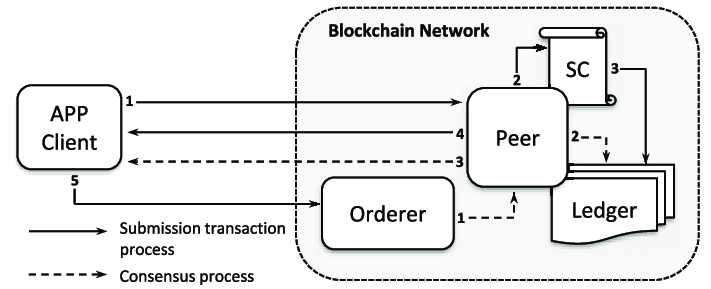
\includegraphics[width=\linewidth]{Graphics/single_node_network.png}
	\caption{Red Hyperledger Fabric de un solo nodo}
	\label{fig:2}
\end{figure}


\subsection{Componentes}

HLF consta de varias componentes principales: nodos peer, orderer y chaincode (ver Figura \ref{fig:2}). Cada componente tiene un rol único para diferentes propósitos.

Los nodos orderer implementan el protocolo de consenso para ordenar las transacciones enviadas por los miembros (clientes) y las clasificará utilizando métodos de consenso. Hyperledger recomienda tres: Solo (dev), kafka, Raft. El ordenador utiliza un protocolo de transmisión atómica para recibir instrucciones de datos. Se detallará un poco más en las componentes del framework

\begin{itemize}
	\item Solo: Recomendado solo para el entorno de desarrollo porque no tiene un sistema tolerante a fallas (se espera que desaparezca en la versión 2.+)
	\item Kafka: Se implementa en varios nodos fuera de los nodos orderer.
	\item Raft: Raft(Reliable, Replicated, Redundant, And Fault-Tolerant) es un servicio de pedidos tolerante a fallas basado en el protocolo Raft en etcd. La principal diferencia con Kafka es que todo está incluido en los nodos de ordenación. Fabric proporciona varios parámetros de configuración, como el tiempo de espera del bloque y el tamaño del bloque en el servicio de pedidos para fines personalizados. 
\end{itemize}

Los nodos Peer son un tipo de nodo que aloja el ledger y el chaincode en el sistema Hyperledger Fabric. Los peer están conectados por canales entre sí y se pueden agrupar según las necesidades para administrar los ledger y los contratos. Los peer pueden ser agrupados por una organización. Juegan dos roles principales en la red: aprobación y confirmación en el ledger. El peer puede tener más de un ledger, que puede ser controlados por uno o mas chaincodes.

Un canal es una subred privada de comunicación entre dos o mas miembros de la red con el objetivo de ejecutar transacciones privadas y confidenciales. Los canales son definidos por las organizaciones, el ledger compartido, el chaincode de la aplicación o el nodo order.

El término chaincode hace referencia a la sección de código que define la lógica aplicada a las transacciones.

\begin{figure}[h!]
	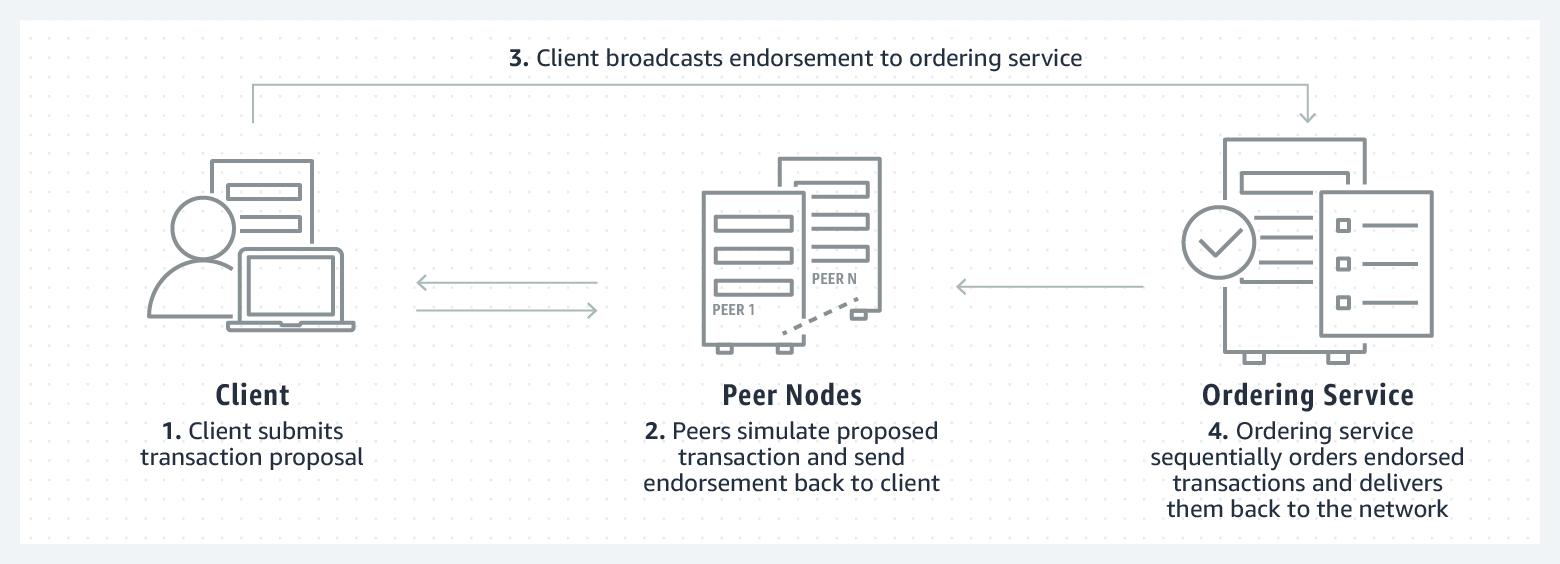
\includegraphics[width=\linewidth]{Graphics/hyp_fab_diagram.png}
	\caption{Flujo simplificado de una transacción en Hyperledger Fabric}
	\label{fig:3}
\end{figure}

\subsection{Flujo}
Para garantizar la coherencia e integridad de los datos, Hyperledger Fabric implementa varios puntos de comprobación en todo el flujo de transacciones, incluidas la autenticación de cliente, aprobación, ordenación y confirmación en el ledger (Figura \ref{fig:3}).

\begin{figure}[h]
	\centering
	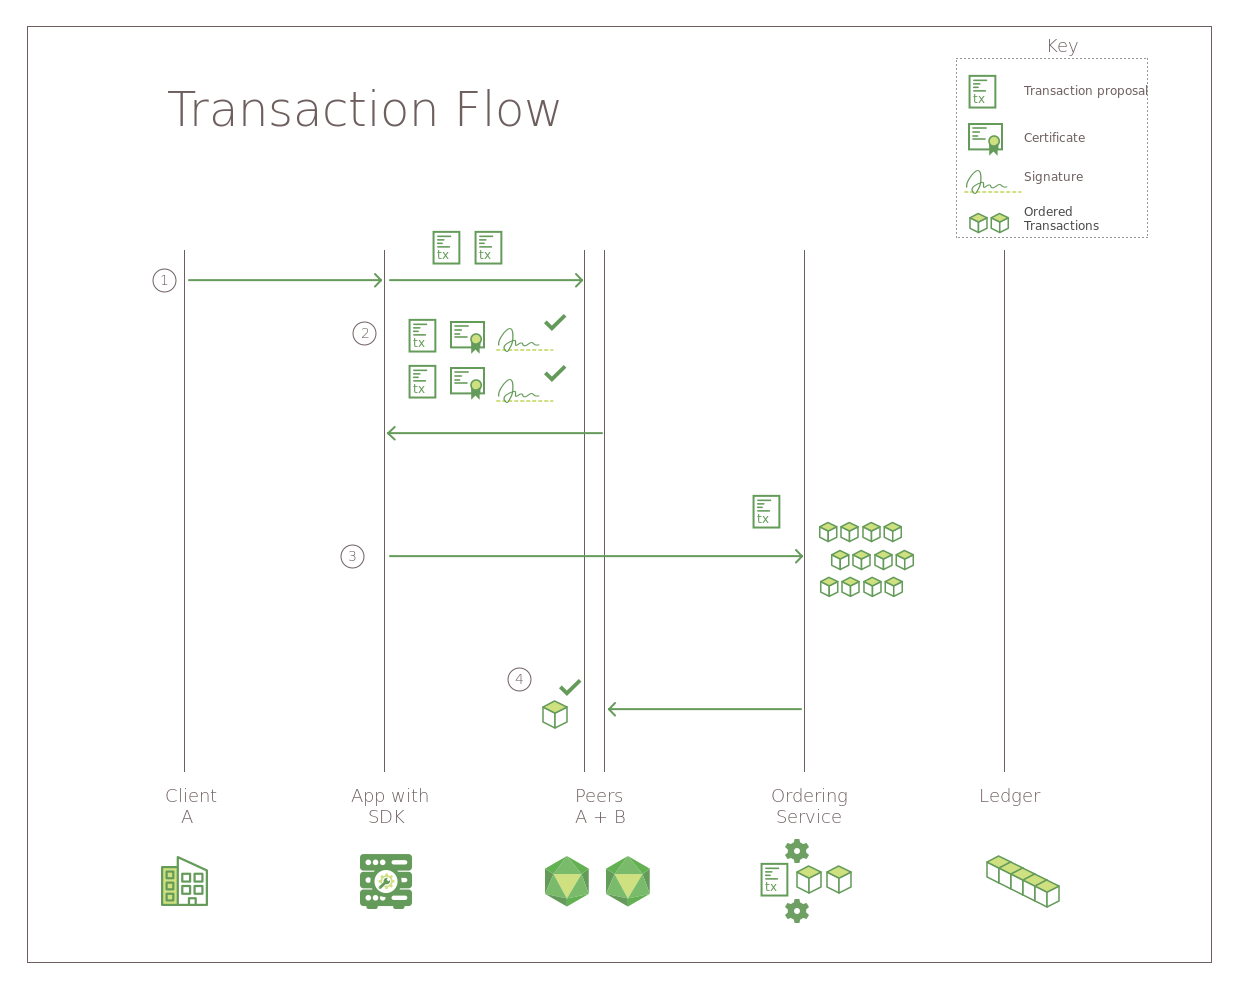
\includegraphics[scale=0.5]{Graphics/txflow.png}
	\caption{Flujo completo de una transacción en Hyperledger Fabric}
	\label{fig:4}
\end{figure}

En una red de Hyperledger Fabric, el flujo de datos (Figura \ref{fig:4}) para consultas y transacciones se inicia desde una aplicación del lado del cliente mediante el envío de una solicitud de transacción a un peer de un canal. El flujo de datos inicial a través de la red es común para ambas:
\begin{enumerate}
	\item Mediante las API disponibles en el SDK, una aplicación cliente firma y envía una propuesta de transacción a los peers de aprobación adecuados en el canal especificado. Esta propuesta de transacción inicial es una solicitud de aprobación.

	\item Cada peer del canal verifica la identidad y la autorización del cliente que realiza el envío y (si es válido) ejecuta el chaincode especificado en las entradas proporcionadas. Según los resultados de la transacción y de la política de aprobación del chaincode invocado, cada peer devuelve a la aplicación una respuesta YES o NO firmada. Cada respuesta YES firmada es una aprobación de la transacción.

	En este punto del flujo de la transacción, el proceso difiere de las consultas y transacciones. Si la propuesta ha invocado una función de consulta en el chaincode, la aplicación devuelve los datos al cliente. Si la propuesta ha invocado una función para actualizar el ledger, la aplicación continúa con los pasos siguientes:

	\item La aplicación reenvía la transacción, que incluye el conjunto de lectura/escritura y las aprobaciones, al servicio de ordenación.
	
	\item Luego la transacción se retransmite al servicio de ordenación. Todos los peers del canal validan las transacciones del bloque mediante la aplicación de la Política de validación específica del chaincode y la ejecución de la comprobación de versiones de control de simultaneidad.
	\begin{itemize}
		\item Las transacciones que no superan el proceso de validación se marcan como no válidas en el bloque y el bloque se añade al ledger del canal.
		\item Todas las transacciones válidas actualizan la base de datos de estado según los pares clave/valor modificados.
	\end{itemize}

\end{enumerate}

El protocolo gossip de diseminación de datos difunde continuamente los datos del ledger a todo el canal para garantizar la sincronización de los ledger de los peers.

\subsection{SDK de Fabric}
Los SDK de Hyperledger Fabric permiten a los desarrolladores de aplicaciones crear aplicaciones que interactúan con una red blockchain. Estos SDK permiten que las aplicaciones gestionen del ciclo de vida de los canales y del código de encadenamiento.

Hyperledger Fabric proporciona un SDK para algunos lenguajes de programación que ofrece las funciones siguientes para la interacción con la red blockchain:

\begin{itemize}
	\item Registrar e inscribir usuarios
	\item Crear canales
	\item Unir peers a un canal
	\item Actualizar la configuración del canal de sistema o canal de aplicación
	\item Instalar chaincode en peers
	\item Crear instancias de chaincode en un canal
	\item Actualizar el chaincode en un canal
	\item Invocar funciones de chaincode para actualizar el ledger
	\item Realizar consultar al ledger sobre transacciones, bloques o claves específicos
	\item Supervisar sucesos de un canal (por ejemplo, la correcta confirmación de una transacción)
\end{itemize}

Para el sistema que se desarrolla en este documento se propone el uso de Go como lenguaje y por tanto se usará el SDK de Go para Hyperledger Fabric. Las razones para escoger Go son la elegancia de su escritura y los resultados que tiene en desempeño.

.

\subsection{Go para escribir Contratos Inteligentes}

Hyperledger Fabric tiene dentro de sus ventajas el uso de contratos inteligentes y mediante el SDK de Fabric se puede escribir la lógica usando lenguajes de programación comunes. Uno de los lenguajes es Go. En esta sección se explica la razón de su uso.

\subsubsection{¿Qué es Go?}
El lenguaje de programación Go es un proyecto de código abierto para hacer que los programadores sean más productivos.

Go es expresivo, conciso, limpio y eficiente. Sus mecanismos de concurrencia facilitan la escritura de programas que aprovechan al máximo las máquinas multinúcleo y en red, mientras que su sistema de tipos permite la construcción de programas modulares y flexibles. Go compila rápidamente en código de máquina pero tiene la comodidad de un Garbage Collector y el poder de la reflexión en tiempo de ejecución. Es un lenguaje compilado, tipificado estáticamente que se siente como un lenguaje interpretado y de tipado dinámico.

\subsubsection{Rendimiento}
Uno de los beneficios más considerables de usar C, C++ sobre otros lenguajes modernos de alto nivel como Java/Python es su rendimiento. La diferencia de rendimiento está en que C/C++ se compilan y no se interpretan. Los procesadores solo entienden binario y los lenguajes interpretados necesitan aplicar más traducciones sobre el código original (Figura \ref{fig:5}). Suele ser común una relación de proporcionalidad inversa entre redibilidad y rendimiento sin embargo go encuentra un punto bastante avanzado en ambos aspectos.

\begin{figure}[h]
	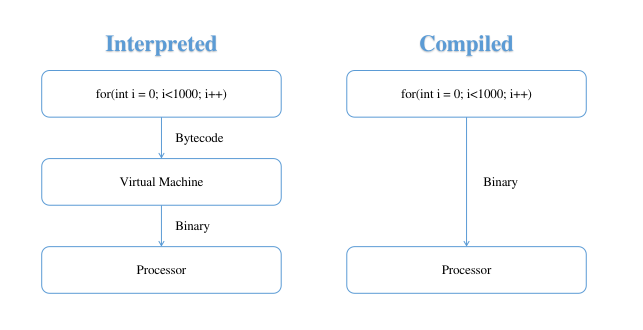
\includegraphics[width=\linewidth]{Graphics/compiled_go.png}
	\caption{Flujo de lenguajes Interpretados vs Compilados}
	\label{fig:5}
\end{figure} 

Otro aspecto que influye en el rendimiento de los lenguajes es como se maneja la liberación y asignación de de variables. En lenguajes compilados son procesos tortuosos, pero evitan tener recursos atendiendo a estos detalles automáticamente. La mayoría de los lenguajes de programación de alto nivel utilizan algoritmos de conteo de referencia o recolector de basura como una capa de abstracción para el desarrollador. Go contiene lo mejor de ambos mundos [\cite{whygo}]


\subsubsection{Concurrencia}
Go es un lenguaje desplegado en 2009 y tiene ventaja sobre lenguajes como Python (desplegado sobre los años 90) en el trabajo multihilos. La ventaja radica en que nace en un contexto donde la idea de concurrencia está más madura. Go incluye los Goroutines que le permite trabajar en paralelo creando estructuras más eficientes en memoria \ref{fig:7}. 

\begin{figure}[h]
	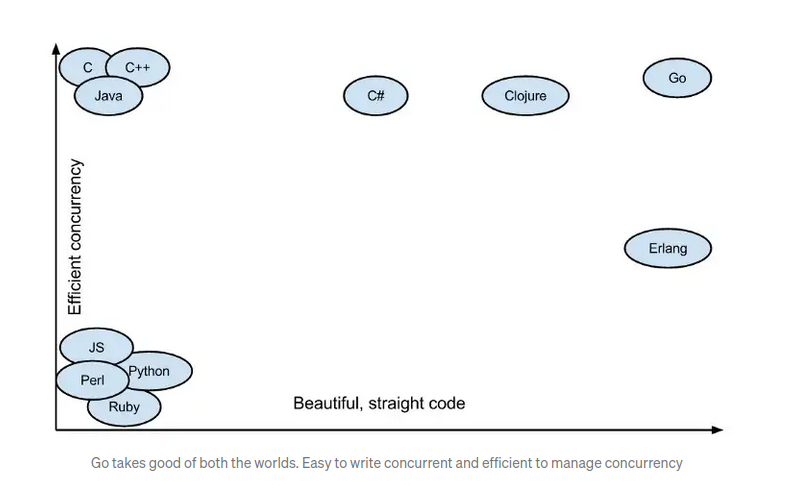
\includegraphics[width=\linewidth]{Graphics/go_concurr.png}
	\caption{Legibilidad del código vs eficiencia de concurrencia}
	\label{fig:7}
\end{figure} 

\subsubsection{Mantenimiento}
Go es un lenguaje pensado para facilitar el mantenimiento del código por futuros programadores. Un ejemplo es el uso de módulos que desacoplan las funcionalidades del programa. Otro aspecto para hacer más sencillo el mantenimiento es la legibilidad. Teniendo en cuenta esto, los desarrolladores de Go diseñaron una sintaxis más agradable y eliminaron elementos del lenguaje como clases y por consiguiente la herencia; anotaciones, excepciones y la genericidad.

\section{Algunas aplicaciones de blockchain en la certificación de documentos}

%Algunos investigadores han empleado blockchain para diseñar diferentes soluciones en el campo de la emisión, el almacenamiento, la verificación de certificados, la financiación y la gestión de derechos digitales [\cite{blockcerts}][\cite{turkanovic2018eductx}][\cite{sharples2016blockchain}][\cite{gazali2017re}][\cite{guo2020blockchain}]. Los documentos podrían compartirse públicamente con terceros de una manera resistente a la pérdida o alteración de datos.

%Sharples y Domingue [\cite{sharples2016blockchain}] propusieron un proyecto en el que los miembros pueden registrarse para aprobar los cursos de formación y recibir fondos. 
%En su proyecto, los esfuerzos científicos de los miembros son recompensados y los registros relacionados se almacenan en una billetera virtual.

%Blockcert [\cite{blockcerts}] es un estándar de código abierto donde diferentes tipos de instituciones pueden unirse a la red. En él no se utilizan contratos inteligentes por lo que un instituto puede emitir un certificado, pero no puede reflejar luego lógica sobre ellos.

%La Universidad de Nicorsia (UNIC) [\cite{kamivsalic2019preliminary}] usa un sistema de certificación que utiliza el esquema Blockcert como diseño básico con algunas modificaciones. UNIC agrupa a los estudiantes que pertenezcan a un curso en particular, de manera q se trabajan siempre como colección. La principal ventaja de este sistema es que reduce el espacio de almacenamiento requerido, a costa de una menor seguridad y privacidad en el acceso a los datos. De manera similar, la Red Nacional de Investigación y Educación de Grecia (GRNET) almacena además los detalles de todo el proceso de verificación en la plataforma Cardano[\cite{castor2018cardano}].

%La aplicabilidad de BCDiploma [\cite{bcdiploma}] y [\cite{turkanovic2018eductx}] es similar entre ellas, excepto que BCDiploma usa contratos inteligentes con un conjunto diferente de estructuras de datos. En BCDiploma, se introduce un sistema para emitir certificados, en la plataforma Ethereum, mediante una URL. El tamaño de los datos en este sistema es un factor importante y hará variar el costo de las transacciones. EduCTX es una plataforma de calificación y crédito en la que se transfieren tokens ECTX (European Credit Transfer and Accumulation System). El ECTX es un sistema estandarizado para comparar créditos académicos en países europeos. Dado que no se utilizan contratos inteligentes, la posibilidad de falsificación o transferencia de la cantidad incorrecta de tokens EduCTX será posible, por lo que se reduce la confiabilidad del sistema.

%UniChain [\cite{daraghmi2019unichain}] emplea contratos inteligentes que gestionan las transacciones y controlan el acceso a los registros académicos electrónicos. Todos los accesos se realizan a través de la blockchain y, en consecuencia, el historial será almacenado. El sistema consta de dos tipos de nodos: estudiantes y universitarios. Los expedientes académicos son encriptados con las claves públicas del nodo universitario así como del nodo estudiante.

%Ocheja et al. [\cite{ocheja2019managing}] presentó un sistema llamado BOLL (the Blockchain of Learning Logs). En trabajos de investigación similares [\cite{guo2020blockchain}][\cite{bore2017towards}] se han presentado soluciones prometedoras para registros basados en cadenas de bloques gestionados por contratos inteligentes, aunque sus contenidos son diferentes. Jungi Guo [\cite{guo2020blockchain}] propuso un sistema de gestión de derechos digitales en un entorno de educación en línea basado en la combinación de blockchains públicas y privadas. Bore [\cite{bore2017towards}] se centró en almacenar valores hash de datos biométricos, documentos, imágenes y cualquier dato multimedia grande en la cadena de bloques

%Algunos autores [\cite{gresch2018proposal}][\cite{karatacs2018developing}][\cite{cheng2018blockchain}][\cite{kumavat2019certificate}] han considerado el uso de contratos inteligentes, pero se han centrado en ciertos procedimientos, como las calificaciones de los estudiantes o la verificación de documentos. Gresch et al. [\cite{gresch2018proposal}] presentó un sistema basado en blockchain mediante el uso de contratos inteligentes en una plataforma de Ethereum llamada UZHBC (University of ZuricH BlockChain).

%Hay otras universidades que han utilizado o pretenden utilizar la tecnología blockchain. Algunos enfoques como Blockcerts, BCDiploma y EduCTX ampliaron la cantidad de emisores en sus redes, mientras que algunos enfoques como UZHBC y UNIC tienen un emisor interno. Algunos proyectos, como EduCTX y UZHBC, solo admiten un tipo de datos, pero otros brindan la capacidad de almacenar todo tipo de credenciales, como BOLL y Blockcert. La mayoría de los proyectos antes mencionados en el ámbito académico se basan en conceptos o ideas cerrados y, a menudo, no discuten los detalles o, sin embargo, permanecen en el nivel de diseño.

Para lograr el objetivo planteado en este trabajo y responder a las preguntas de investigación, se realizó un estudio sobre el uso de la tecnología blockchain en el sector educativo, específicamente en la emisión de diplomas a los graduados universitarios.

\subsection{Certificados digitales en universidades}
Actualmente, algunas universidades alrededor del mundo han adoptado varias técnicas para dar servicios de emisión  y verificación de certificados digitales como la Universidad de Johannesburgo (UJ) en Sudáfrica [\cite{80}], la Universidad de Exeter [\cite{76}], y otras más [\cite{1}].

Todos los certificados que emite la Universidad de Johannesburgo (UJ) incluyen códigos QR basados en \textit{blockchain}. 

La Universidad de Exeter lanzó una pequeña aplicación piloto para su curso de Maestría en Tecnología Financiera [\cite{76}]. El piloto permitió a los estudiantes poseer su certificación sin depender de terceros. Los estudiantes ahora pueden ``propietarios'' de sus certificados y demostrar que la Universidad de Exeter emite un diploma certificado por una \textit{blockchain}.

\subsection{BCdiploma}
Implementado en más de 90 instituciones en una docena de países, BCdiploma (\textit{Blockchain Certified diploma}) [\cite{75}] ofrece un servicio llave en mano para crear y compartir certificados de \textit{blockchain} para variados documentos académicos: como títulos, diplomas, transcripciones o habilidades adquiridas.

Desde enero de 2021 [\cite{75, 78}], los graduados de Montpellier Business School reciben una versión digital de su diploma, una credencial digital emitida con la solución BCdiploma.

La escuela de negocios ESCP (Escuela Superior de Comercio de París) [\cite{74}] lanzó su servicio de credenciales digitales basado en blockchain en asociación con BCdiploma [\cite{75}]. La asociación con BCdiploma simplificó el acceso a los documentos, pues se puede acceder a los diplomas con pocas interacciones, ya sea desde una computadora o un teléfono inteligente.

La Agencia Universitaria de la Francofonía (AUF), en colaboración con BCdiploma, ofrece una solución de certificación \textit{blockchain} a sus universidades [\cite{77}]. La oferta exclusiva firmada con BCdiploma permite a la red de universidades miembro de AUF y sus socios emitir certificados en línea multilingües a prueba de manipulaciones con solo unos pocos clics, que se pueden compartir en redes profesionales y currículums. Los graduados reciben un enlace URL único y seguro que pueden usar libremente de por vida.

La solución BCdiploma presenta una interfaz simple y sencilla. Los emisores de certificados, sean estos la institución, una universidad o facultad, por ejemplo, pueden cargar sus diplomas con la DApp BCdiploma. El almacenamiento del diploma genera un enlace url único y seguro que la institución puede enviar de forma segura al graduado en cuestión. Los graduados pueden compartir la url por correo electrónico, o en las redes sociales. Con ese enlace es posible la visualización de datos (diplomas multilingües) del graduado, y cualquier tercero puede verificar la autenticidad del documento este. 

\subsection{Blockcerts}
La aplicación Blockcerts Wallet fue desarrollada por Learning Machine en conjunto con la Oficina de Registro del MIT [\cite{81, 79}]. Utiliza la tecnología blockchain para brindar a los graduados un fácil acceso a una versión verificable y a prueba de manipulaciones de su diploma que pueden compartir con posibles empleadores. % [\cite{79}].

Una vez que el estudiante descarga la aplicación móvil, genera el par de claves pública y privada y envía la clave pública al MIT, donde se escribe en el registro digital. A continuación, se agrega a la cadena de bloques un hash unidireccional (una cadena de números que se pueden usar para la verificación posteriormente). La información del diploma no se guarda en la cadena de bloques, solo la transacción con marca de tiempo que indica que el MIT creó el registro digital. Finalmente, el MIT envía por correo electrónico el diploma digital (un archivo de notación de objetos de JavaScript o JSON) con la clave pública del estudiante inscrita en el archivo. Debido a que la aplicación móvil en el teléfono del estudiante tiene su clave privada única, el estudiante puede probar la propiedad del diploma.

\subsection{Certifaction}
El sistema de nombre Certifaction ofrece una solución fácil y rápida para asegurar los diplomas de los estudiantes en \textit{blockchain} Ethereum, lo cual los hace inmutables y verificables al instante. El Centro de Finanzas Innovadoras de la Universidad de Basilea y la Universidad de St. Gallen son instituciones que implementan directamente la API de Certifaction en su sistema de emisión de diplomas [\cite{82}].

\subsection{BlockTac}
Con BlockTac [\cite{83}] la institución educativa emite un certificado y lo comunica a BlockTac a través de un canal privado. BlockTac notifica al estudiante y facilita una aplicación de Android o iOS para ver su certificado. El estudiante puede compartir desde la aplicación su certificado con quien desee y cualquier persona o institución puede verificar el certificado sin tener que contactar a la institución acreditadora.

\subsection{Certif-ID}
Certif-ID proporciona un sistema integral para emitir certificados digitales en un formato seguro de cadena de bloques que se puede compartir y verificar instantáneamente en cualquier parte del mundo [\cite{84}]. Certif-ID permite crear, emitir y diseñar certificados, y compartirlos en las redes sociales. Es posible realizar la verificación con tan solo un clic y  rastrear todos los certificados emitidos y compartidos.

\subsection{Emercoin}
Emercoin desarrolló una innovadora plataforma blockchain ``Trusted Diploma'' [\cite{87}] que ayuda a las escuelas a crear y compartir diplomas y otros certificados educativos en una aplicación cifrada. Los registros se almacenan en la \textit{blockchain} y cualquier persona puede verificarlos fácilmente. Flexibilidad, facilidad de uso y disponibilidad son las principales ventajas de esta solución tecnológica.

TruScholar [\cite{86}], CertifyMe.Online [\cite{85}], Credly [\cite{89}] son también soluciones para crear, emitir y administrar credenciales digitales. Ellas poseen interfaces simples e intuitivas que permiten realizar sus operaciones con unos pocos clics en cuestión de minutos.

\subsection{Certika}
Certika es una plataforma web que permite certificar cualquier documento digital de valor bajo tecnología blockchain [\cite{88}]. Para crear un certificado solo es necesario subir la imagen y llenar los campos solicitados (nombres, descripción, habilidades, criterios, atributos, entre otros). La funcionalidad de emitir certificados en esta plataforma es muy sencilla, se debe descargar un archivo CSV y llenar los campos requeridos, los cuales corresponden a la información de los usuarios receptores. Luego, se sube el archivo y el sistema se encargará de emitir un correo a cada persona. En este módulo se podrá agrupar las distintas emisiones realizadas, adicionalmente editar el nombre asignado a los diferentes grupos de certificados, enviar correos de recordatorio a los usuarios receptores, descargar bases de datos y revocar la emisión en caso de haber cometido algún error.

\subsection{Universidad de Ciego de Ávila}
La plataforma UniLegal, de la Universidad de Ciego de Ávila Máximo Gómez Báez (Unica) le permite a los egresados de esa casa de altos estudios la validación de la copia de sus títulos universitarios, a través de dispositivos móviles o computadoras capaces de conectarse a la red nacional, según el periódico Invasor [\cite{90}]. Aunque esta plataforma no está basada en \textit{blockchain}, es válida de mención como antecedente de una plataforma de emisión y validación de títulos universitarios en nuestro país.

Para su uso, el sitio precisa, en un primer momento, del registro del interesado mediante la introducción de datos como su nombre y apellidos, correo electrónico y número del carné de identidad, este último de gran importancia para garantizar la veracidad de la información aportada. Una vez registrado, el interesado podrá subir a la plataforma una fotocopia del título universitario, a la que se le coloca por detrás toda la información registrada en el original y se confronta con el documento aportado para comprobar su validez. La aplicación genera un código de barras y un QR que, al escanearlo, remite a una página donde aparecen los datos específicos del usuario en cuestión y a la cual puede acceder cualquier persona para verificar que ese documento sea verdadero.


